\newpage
\section{Specifica del prodotto}
In questa sezione verrà descritta in maniera macroscopica l'architettura che verrà adottata nella progettazione. Per semplificare la comprensione, verrà utilizzato un approccio top-down partendo dalle linee generali fino a giungere ad una descrizione in dettaglio delle componenti.

\subsection{Architettura generale}
Il software API Market si caratterizza dalle comuni applicazioni per l'approccio a Microservizi adottato nell'implementazione. In maniera differente da un applicazione monolitica, ogni componente viene realizzato come microservizio a sè stante. L'aggregazione di questi microservizi definisce l'applicazione finale e ne realizza il comportamento definitivo. Esulando dall'approccio a microservizi, il sistema sarà realizzato al pari di una classica applicazione \textit{Client-Server}, dove il lato Front-end (Client) si occuperà di fornire all'utente finale l'interfaccia web su cui poter interagire, mentre il lato Back-end (Server) gestirà e salverà i dati, e si occuperà della gestione delle chiamate API (Tramite l'opportuna componente \textit{API Gateway}). La base di dati utilizzata si occupa della raccolta di dati sensibili dell'utenza, gestione delle applicazioni e chiavi e gestione dei dati statistici.

Il sistema verrà realizzato, per il lato back-end, tramite microservizi con interfaccia Jolie che verranno implementati con codice Java. Questo approccio, sebbene la tematica sia di recente sviluppo, risulta molto gettonato dalle grandi realtà che si sono affacciate a questo approccio (come ad esempio l'AWS Service registry "Eureka" usato dalla piattaforma Netflix). Il lato front-end invece verrà implementato tramite HTML e Javascript, in particolare l'utilizzo del framework full-stack MeteorJS consentirà un binding in real-time per la rappresentazione delle informazioni.
Nella realizzazione dell'API Market richiesto verrà utilizato il desing pattern Model View ViewModel; alcune componenti di questo pattern addotteranno un design patterna microservizi, espresso in due varianti, a catena e di aggregazione.
\begin{figure}[H]
	\centering
	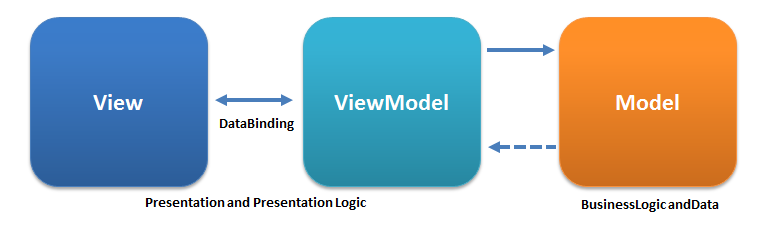
\includegraphics[width=0.7\linewidth]{IMG/MVVMPattern}
	\caption{Il design pattern Model View ViewModel}
\end{figure}

\subsubsection{Pattern architetturale front-end}
Il design pattern Model View ViewModel è suddiviso in tre componenti, ed in questa porzione andremo a spiegare brevemente la funzionalità di ognuna. Verrà motivata inoltre la scelta di tale pattern da parte del gruppo.

\begin{itemize}
	\item \textbf{Model}: rappresenta il punto di accesso ai dati, si occupa dell'interazione con essi e ne specifica le modalità di accesso. Nella definizione dell'API Market il model si trova nel Back-end;
	\item \textbf{View}: la view è in grado di gestire eventi, eseguire operazioni ed effettuare il data-binding;
	\item \textbf{ViewModel}: il ViewModel è  il punto di incontro tra la View e il Model: i dati ricevuti da quest’ultimo sono elaborati per essere presentati e passati alla View.
\end{itemize}

In fase di progettazione il gruppo ha preso in esame diversi design pattern architetturali, ma la volontà di realizzare pagine web dinamiche e reattive, unitamente all'uso di tecnologie quali AngularJS e il sistema di comunicazione MeteorJS hanno indirizzato la scelta verso il pattern MVVM.

\paragraph{Componente Model}
Il Model è situato nella parte lato server del sistema e svolge le seguenti funzioni:
\begin{itemize}
	\item Interagisce con i database nei quali vengono salvati i dati del sistema, come API, transazioni e profili di utenti. Le funzionalità incluse comprendono microservizi in grado di caricare, salvare, modificare e cancellare dati sui database;
	\item Offre un'interfaccia logica di accesso al ViewModel attraverso la quale richiedere dati e operazioni su di essi, tramite funzionalità del framework Meteor come il Publishing e Subscribing.
\end{itemize}
\paragraph{Componente View}
La componente View è situata nella parte front-end del sistema e ha lo scopo di:
\begin{itemize}
	\item Rappresentare i dati del ViewModel e non interagisce in nessun modo con essi;
	\item Visualizzare le funzionalità offerte all'utente.
\end{itemize} 
La componente View è una interfaccia web, ed il gruppo ha scelto di utilizzare CSS3 e HTML5 per le parti statiche, mentre verrà utilizzato AngularJS per le parti dinamiche. 
\paragraph{Componente ViewModel}
La componente ViewModel è situata nella parte front-end del sistema e comunica sia con la View sia con il Model. Esso è l'unico componente a conoscere gli altri, realizzando un totale disaccopiamento tra la View e il Model. Il ViewModel ha tre compiti fondamentali, ovvero:
\begin{itemize}
	\item Realizzare il data-binding;
	\item Passare gli input della View e tradurli in azioni Model;
	\item Richiedere i dati al Model tramite la tecnica \textit{Publish-Subscribe} di MeteorJS e inviarli alla View.
\end{itemize}

\subsubsection{Pattern architetturale back-end}
All'interno della componente Model sono presenti una serie di microservizi relizzati con il design pattern Aggregator Microservice. 
\begin{figure}[H]
	\centering
	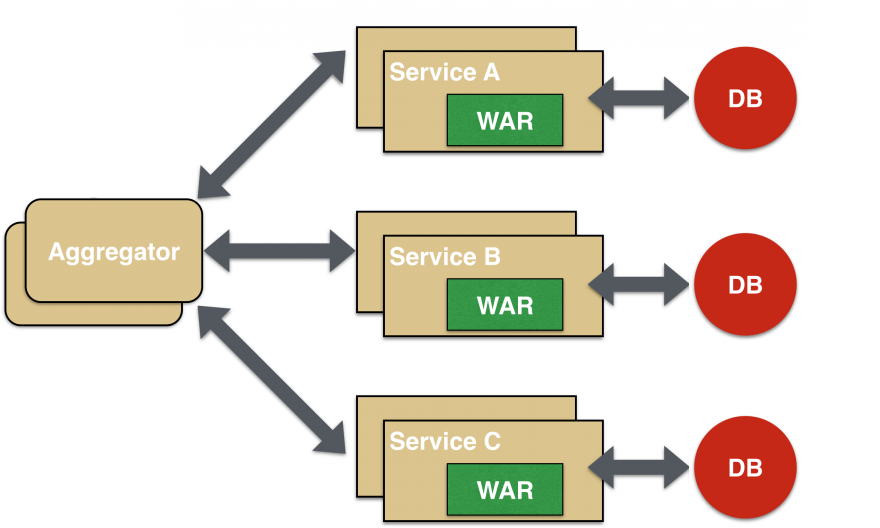
\includegraphics
	[width=0.7\linewidth]
	{IMG/microservices-aggregator}
	\caption{Aggregator Microservices design pattern}
\end{figure}
Questo design pattern si compone di un aggregatore, ovvero un microservizio in grado di collezionare i dati che gli vengono forniti da diversi microservizi, per poi renderli fruibili all'utente tramite la componente View. Utilizzando un design pattern a microservizi è necessario che le varie componenti siano indipendenti tra di loro e quindi che anche i relativi database lo siano. La realizzazione di un unico database avrebbe portato alla realizzazione di una architettura SOA, ovvero una architettura orientata ai servizi. Tutti i microservizi contenuti in un package, sono indipendenti da microservizi contenuti in altri package ed ogni microservizio opera sul database associato.

\subsubsection{Pattern architetturale API Gateway}
Il design pattern architetturale scelto per l'API Gateway è il Design pattern a Microservizi concatenato. Questo tipo di pattern è una sequenza di azioni prestabilite innescate da una richiesta HTTP. 
\begin{figure}[!h]
	\centering
	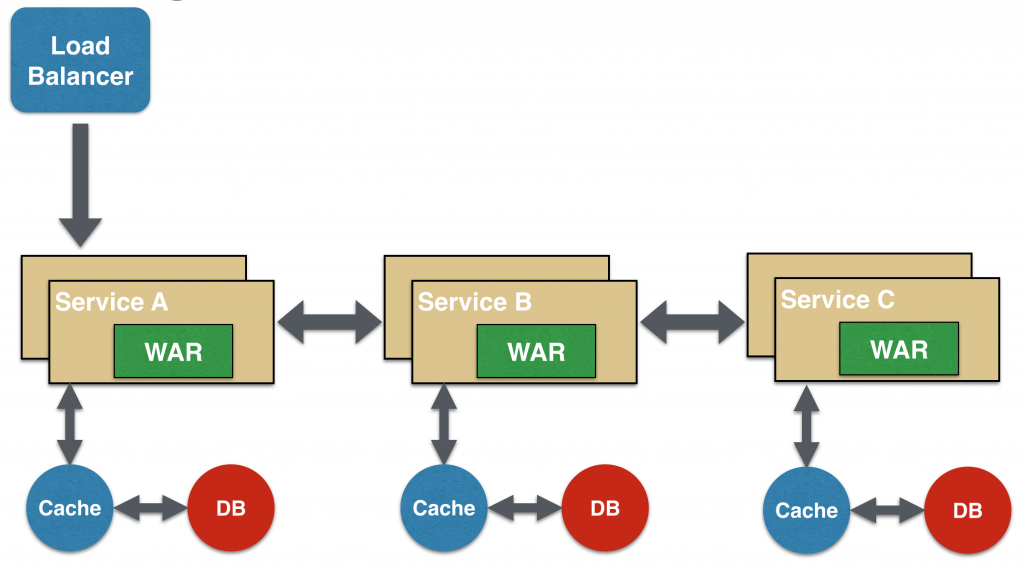
\includegraphics
	[width=0.7\linewidth]
	{IMG/microservices-chain}
	\caption{Chained Microservice Design Pattern}
\end{figure}
Ogni servizio non può intraprendere la propria esecuzione se non è terminato il servizio precedente. Un punto critico di questa scelta è la lunghezza della catena. L'API Gateway è progettato per elaborare una richiesta e ritornare una risposta al chiamante, trattandosi dunque di domande sincrone. Una catena troppo lunga crea una tempo di attesa non indifferente per il client, considerando che bisogna valutare anche il tempo impiegato dal microservizio target della chiamata all'API Gateway.

\subsubsection{SOA vs. Microservices Architecture}
In sede di scelta architetturale, il gruppo NetBreak ha analizzato le principali architetture in materia di microservizi. L'architettura \textit{Service Oriented Architecture} è una scelta intermedia tra le applicazioni monolitiche e le applicazioni completamente a microservizi. In una \textit{SOA}, l'applicazione è composta da una sorta di collezione di servizi. L'applicazione base viene quindi scomposta in una collezione di servizi. L’approccio a microservizi tende, invece, alla realizzazione di una singola applicazione composta da un numero arbitrario di servizi. Essi vengono quindi sviluppati e implementati in maniera indipendente. Tale approccio presenta un alto livello di flessibilità e scalabilità, predisponendo la massima indipendenza dei componenti (microservizi). Un esempio è la scelta di utilizzo del database citata precedentemente: nella traduzione di un applicazione da monolitica (oppure SOA) ad un architettura a microservizi, il database viene scomposto in parti indipendenti. La comunicazione tra i servizi è basata su HTTP tramite le API RESTful, passando i dati in formato JSON: nello specifico caso del nostro applicativo, la comunicazione sarà gestita su un diverso livello di astrazione tramite i framework MeteorJS e AngularJS che si occuperanno della trasmissione dati in formato JSON con maggior autonomia.
